\documentclass[]{book}
\usepackage{lmodern}
\usepackage{amssymb,amsmath}
\usepackage{ifxetex,ifluatex}
\usepackage{fixltx2e} % provides \textsubscript
\ifnum 0\ifxetex 1\fi\ifluatex 1\fi=0 % if pdftex
  \usepackage[T1]{fontenc}
  \usepackage[utf8]{inputenc}
\else % if luatex or xelatex
  \ifxetex
    \usepackage{mathspec}
  \else
    \usepackage{fontspec}
  \fi
  \defaultfontfeatures{Ligatures=TeX,Scale=MatchLowercase}
\fi
% use upquote if available, for straight quotes in verbatim environments
\IfFileExists{upquote.sty}{\usepackage{upquote}}{}
% use microtype if available
\IfFileExists{microtype.sty}{%
\usepackage{microtype}
\UseMicrotypeSet[protrusion]{basicmath} % disable protrusion for tt fonts
}{}
\usepackage{hyperref}
\hypersetup{unicode=true,
            pdftitle={Proctor Foundation Data Science Handbook},
            pdfauthor={Contributors (many from UC Berkeley in addition to Proctor): Ben Arnold, Jade Benjamin-Chung, Kunal Mishra, Stephanie Djajadi, Nolan Pokpongkiat},
            pdfborder={0 0 0},
            breaklinks=true}
\urlstyle{same}  % don't use monospace font for urls
\usepackage{natbib}
\bibliographystyle{apalike}
\usepackage{longtable,booktabs}
\usepackage{graphicx,grffile}
\makeatletter
\def\maxwidth{\ifdim\Gin@nat@width>\linewidth\linewidth\else\Gin@nat@width\fi}
\def\maxheight{\ifdim\Gin@nat@height>\textheight\textheight\else\Gin@nat@height\fi}
\makeatother
% Scale images if necessary, so that they will not overflow the page
% margins by default, and it is still possible to overwrite the defaults
% using explicit options in \includegraphics[width, height, ...]{}
\setkeys{Gin}{width=\maxwidth,height=\maxheight,keepaspectratio}
\IfFileExists{parskip.sty}{%
\usepackage{parskip}
}{% else
\setlength{\parindent}{0pt}
\setlength{\parskip}{6pt plus 2pt minus 1pt}
}
\setlength{\emergencystretch}{3em}  % prevent overfull lines
\providecommand{\tightlist}{%
  \setlength{\itemsep}{0pt}\setlength{\parskip}{0pt}}
\setcounter{secnumdepth}{5}
% Redefines (sub)paragraphs to behave more like sections
\ifx\paragraph\undefined\else
\let\oldparagraph\paragraph
\renewcommand{\paragraph}[1]{\oldparagraph{#1}\mbox{}}
\fi
\ifx\subparagraph\undefined\else
\let\oldsubparagraph\subparagraph
\renewcommand{\subparagraph}[1]{\oldsubparagraph{#1}\mbox{}}
\fi

%%% Use protect on footnotes to avoid problems with footnotes in titles
\let\rmarkdownfootnote\footnote%
\def\footnote{\protect\rmarkdownfootnote}

%%% Change title format to be more compact
\usepackage{titling}

% Create subtitle command for use in maketitle
\providecommand{\subtitle}[1]{
  \posttitle{
    \begin{center}\large#1\end{center}
    }
}

\setlength{\droptitle}{-2em}

  \title{Proctor Foundation Data Science Handbook}
    \pretitle{\vspace{\droptitle}\centering\huge}
  \posttitle{\par}
    \author{Contributors (many from UC Berkeley in addition to Proctor): Ben Arnold, Jade Benjamin-Chung, Kunal Mishra, Stephanie Djajadi, Nolan Pokpongkiat}
    \preauthor{\centering\large\emph}
  \postauthor{\par}
      \predate{\centering\large\emph}
  \postdate{\par}
    \date{2019-10-01}

\usepackage{booktabs}

\begin{document}
\maketitle

{
\setcounter{tocdepth}{1}
\tableofcontents
}
\hypertarget{welcome}{%
\chapter*{Welcome!}\label{welcome}}
\addcontentsline{toc}{chapter}{Welcome!}

Welcome to the Francis I. Proctor Foundation at the University of California, San Francisco (\url{https://proctor.ucsf.edu})!

This handbook summarizes some best practices for data science, drawing from our experience at the Francis I. Proctor Foundation and from that of our close colleagues in the Division of Epidemiology and Biostatistics at the University of California, Berkeley (where Prof.~Ben Arnold worked for many years before joining Proctor).

We do not intend this handbook to be a comprehensive guide to data science. Instead, it focuses more on practical, ``how-to'' guidance for conducting data science within epidemiologic research studies. Although many of the ideas of environment-independent, the examples draw from the \href{https://cran.r-project.org/}{R} programming language. For an excellent overview of data science in R, see the book \href{https://r4ds.had.co.nz/}{R for Data Science}.

Much of the material in this handbook evolved from a version of Dr.~Jade Benjamin-Chung's \href{https://github.com/jadebc-berkeley/lab-manual}{lab manual} at the University of California, Berkeley. In addition to the Proctor team, many contributors include current and former students from UC Berkeley.

The last two chapters of the handbook cover our communication strategy and code of conduct for team members who work with Prof.~Ben Arnold, who leads Proctor's Data Coordinating Center. They summarize key pieces of a functional data science team. Although the last two chapters might be of interest to a broader circle, \emph{they are mostly relevant for people working directly with Ben.} Just because they are at the end does not make them less important.

It is a living document that we strive to update regularly. If you would like to contribute, please write Ben (\href{mailto:ben.arnold@ucsf.edu}{\nolinkurl{ben.arnold@ucsf.edu}}) and/or submit a pull request.

The GitHub repository for this handbook is: \url{https://github.com/proctor-ucsf/dcc-handbook}

\hypertarget{intro}{%
\chapter{Introduction: Work Flow and Reproducible Analyses}\label{intro}}

\emph{Contributors: Ben Arnold}

This handbook collates a number of tips to help organize the workflow of epidemiologic data analyses. There are probably a dozen good ways to organize a workflow for reproducible research. This document includes recommendations that arise from our own team's experience through numerous field trials and observational data analyses. The recommendations will not work for everybody or for all applications. But, they work well for most of us most of the time, else we wouldn't put in the time to share them.

Start with two organizing concepts:

\begin{itemize}
\item
  \textbf{Workflow}. Defined here as the process required to draw scientific inference from data collected in the field or lab. I.e., the process by which we take data, and then process it, share it internally, analyze it, and communicate results to the scientific community.
\item
  \textbf{Reproducible research}. A fundamental characteristic of the scientific method is that study findings can be reproduced beyond the original investigators. Data analyses that contribute to scientific research should be described and organized in a way that they could be reproduced by an independent person or research group. A data analysis that is not reproducible violates a core principle of the scientific method.
\end{itemize}

\hypertarget{workflow}{%
\section{Workflow}\label{workflow}}

Broadly speaking, a typical scientific data science work flow involves four steps to transform raw data (e.g., from the field) into summaries that communicate results to the scientific community.

\begin{figure}
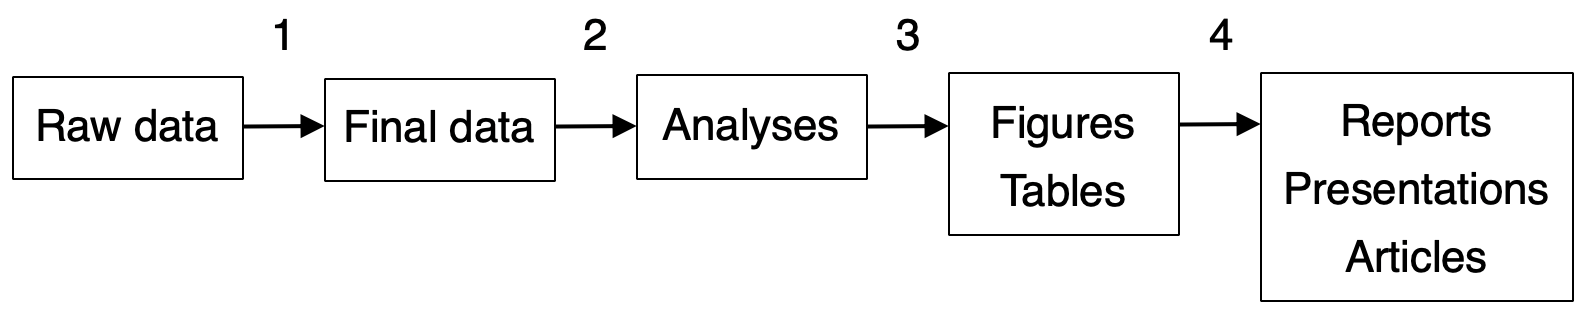
\includegraphics[width=0.75\linewidth]{/Users/benarnold/dcc-handbook/images/workflow} \caption{Overview of the four main steps in a typical data science workflow}\label{fig:fig-workflow}
\end{figure}

When starting a new project, the work flow tends to evolve gradually and by iteration. Data cleaning, data processing, exploratory analyses, back to data cleaning, and so forth. If the work takes place in an unstructured environment with no system to organize files and work flow, it rapidly devolves into into a disorganized mess; analyses become difficult or impossible to replicate and they are anything but scientific. Projects with short deadlines (e.g., proposals, conference abstract submissions, article revisions) are particularly vulnerable to this type of organizational entropy. Putting together a directory and workflow plan from the start helps keep files organized and prevent disorder. Modifications are inevitable -- as long as the system is organized, modifications are usually no problem.

Depending on the project, each step involves a different amount of work. Step 1 is by far the most time consuming, and often the most error-prone. We devote an entire chapter to it below (\protect\hyperlink{datacleaning}{Data cleaning and processing})

\hypertarget{reproducibility}{%
\section{Reproducibility}\label{reproducibility}}

As a guiding directive, this process should be reproducible. If you are not familiar with the concept of reproducible research, start with this manifesto (\href{https://www.nature.com/articles/s41562-016-0021}{Munafo et al.~2017}). For a deeper dive, we highly recommend the recent book from Christensen, Freese, and Miguel (\href{https://www.ucpress.edu/book/9780520296954/transparent-and-reproducible-social-science-research}{2019}). Although it is framed around social science, the ideas apply generally.

\hypertarget{automation}{%
\section{Automation}\label{automation}}

We recommend that the workflow be as automated as possible using a programming language. Automating the workflow in a programming language, and essentially reducing it to text, is advantageous because it makes the process transparent, well documented, easily modified, and amenable to version control; these characteristics lend themselves to reproducible research.

At Proctor, we mostly use R. With the development of \href{https://rstudio.com/}{Rstudio}, \href{https://rmarkdown.rstudio.com/}{R Markdown} and the \href{https://www.tidyverse.org/}{tidyverse} ecosystem (among others), the R language has evolved as much in the past few years as in all previous decades since its inception. This has made the conduct of automated, reproducible research considerably easier than it was 10 years ago.

\textbf{If you have a step in your analysis workflow that involves point-and-click or copy/paste, then STOP, and ask yourself (and your team): } \textbf{\emph{How can I automate this?}}

\bibliography{book.bib,packages.bib}


\end{document}
